\section{Results and Discussion}\label{section:result}

% =====================================================================
%   Five experimental subsections + summary. Each subsection asks one
%   question, answers it with one inline figure (also archived in the
%   appendix), and closes with a short discussion paragraph.
%   Sign convention for the scaled approximation ratio follows
%   \cref{eq:approxratio}: r = (E_worst - E)/(E_worst - E_opt).
% =====================================================================

The five subsections below sweep one design knob at a time on the canonical $n=16$ universe of \cref{section:impl}, fixing the others at $p=3$, $K=4$, $\lambda=2.0$, $A=0.5$, ten COBYLA multi-starts and a statevector backend. Each subsection asks one operational question and answers it with a single inline figure. Throughout we quote the scaled approximation ratio
\begin{equation*}
    r \;=\; \frac{E_{\text{worst}} - E}{E_{\text{worst}} - E_{\text{opt}}} \;\in\; [0,1]
\end{equation*}
of \cref{eq:approxratio} alongside the unscaled relative gap $\mathrm{gap} = (E - E_{\text{opt}})/|E_{\text{opt}}|$; as the sweeps will show, the two metrics disagree often enough that neither suffices on its own.


\subsection{QAOA on the canonical instance}\label{subsec:single-run-results}

How does a single QAOA run perform on the $n=16$ benchmark, and where on the cost spectrum does it actually land? \Cref{fig:single-run} shows the converged energy per restart and the measurement distribution of the best run.

\begin{figure*}[t]
    \centering
    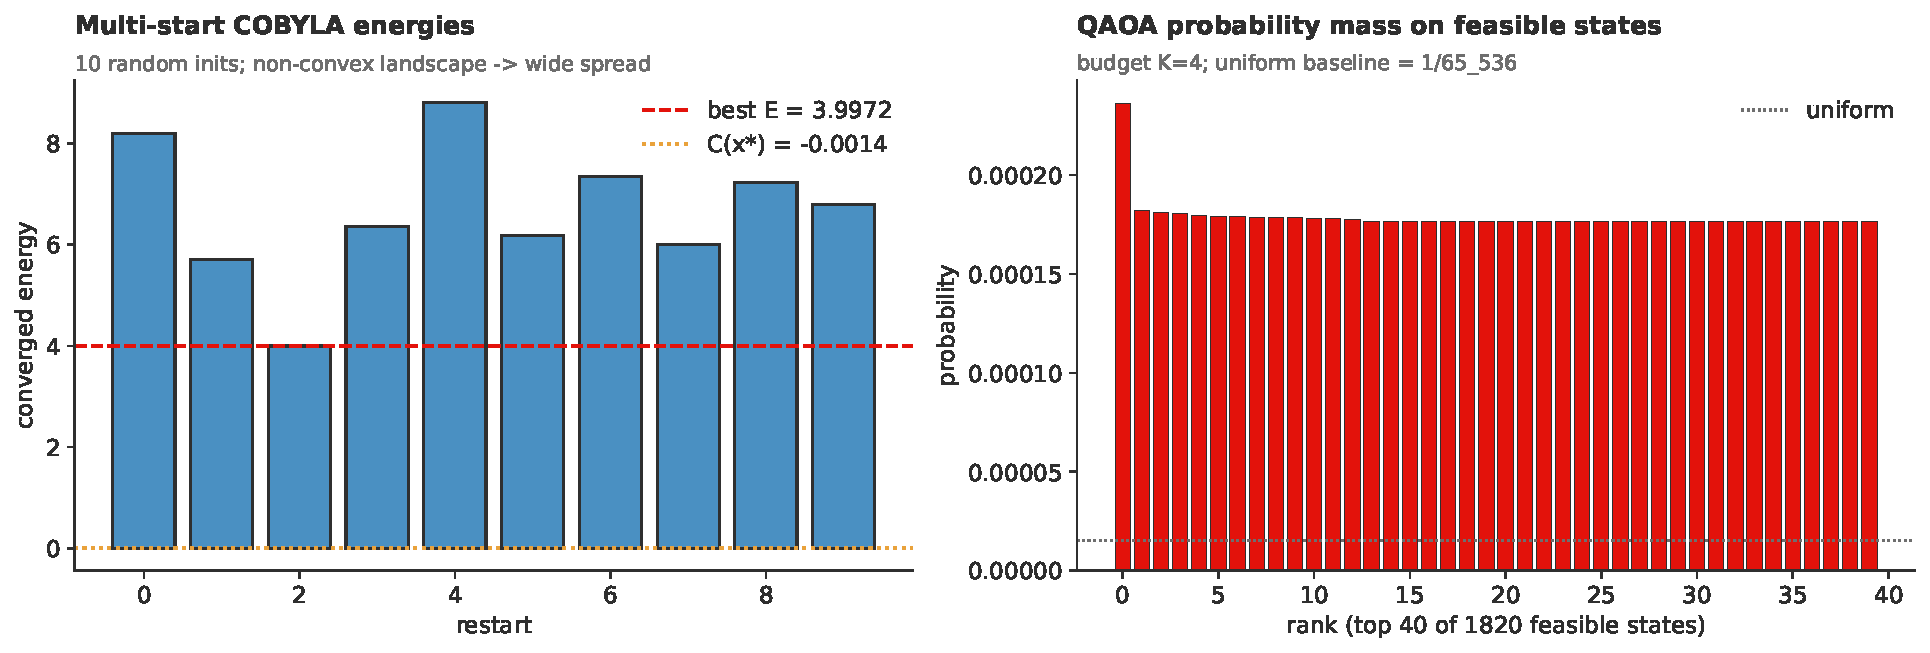
\includegraphics[width=0.8\textwidth]{plots/qaoa/single_run_universe_p3.pdf}
    \caption{Canonical instance ($n=16$, $K=4$, $p=3$, $\lambda=2.0$, $A=0.5$, ten random COBYLA multi-starts, statevector backend). Left: final converged energy per restart, with the brute-force optimum $E_{\text{opt}} = -1.4\times 10^{-3}$ marked as a horizontal line; the spread illustrates the non-convex variational landscape and how often the optimiser settles well above the optimum. Right: probability mass on the top-40 of $\binom{16}{4} = 1820$ budget-feasible bitstrings, plotted against the uniform baseline $1/2^{16} \approx 1.5\times 10^{-5}$.}
    \label{fig:single-run}
\end{figure*}

The best of ten restarts converges to $E = 4.00$ on a cost spectrum bounded below by $E_{\text{opt}} = -1.40\times 10^{-3}$ and above by $E_{\text{worst}} = 72.2$. By the scaled metric this is $r = 0.945$, a number that looks reassuring on its own. The unscaled relative gap, however, is $\mathrm{gap} = 2847$: the variational state's mean energy is nearly three thousand times the optimum. The denominator of $r$ is dominated by the budget penalty $AK^2$, which inflates $E_{\text{worst}}$ from the small return/risk scale to order ten and compresses the population of plausible bitstrings into a narrow band near the top of $[0,1]$ --- a measurement-side artefact also flagged by \textcite{stopfer2025benchmark} on different portfolio benchmarks. The right panel quantifies the measurement story: $p_{\text{opt}} = 1.6\times 10^{-4}$, only about ten times the uniform baseline $1/2^{16} \approx 1.5 \times 10^{-5}$, while $p_{\text{feas}} = 0.31$ is roughly two thousand times what uniform sampling would give. The variational state is feasibility-biased but not optimum-concentrated: the algorithm has learnt the cardinality constraint encoded in $A$ much better than the return/risk landscape encoded in $(\boldsymbol\mu, \boldsymbol\Sigma)$, the failure mode one expects when the penalty dominates the spectrum. We retain this point as the reference against which the four sweeps below vary one knob at a time.


\subsection{Energy landscape at $p=1$}\label{subsec:landscape-results}

What does the variational energy surface $E(\gamma,\beta)$ of \cref{eq:Egb} actually look like? Mapping it on a grid is only feasible at $p=1$, where the surface is two-dimensional; \cref{fig:landscape} shows the contour plot on the canonical $n=16$ instance.

\begin{figure*}[t]
    \centering
    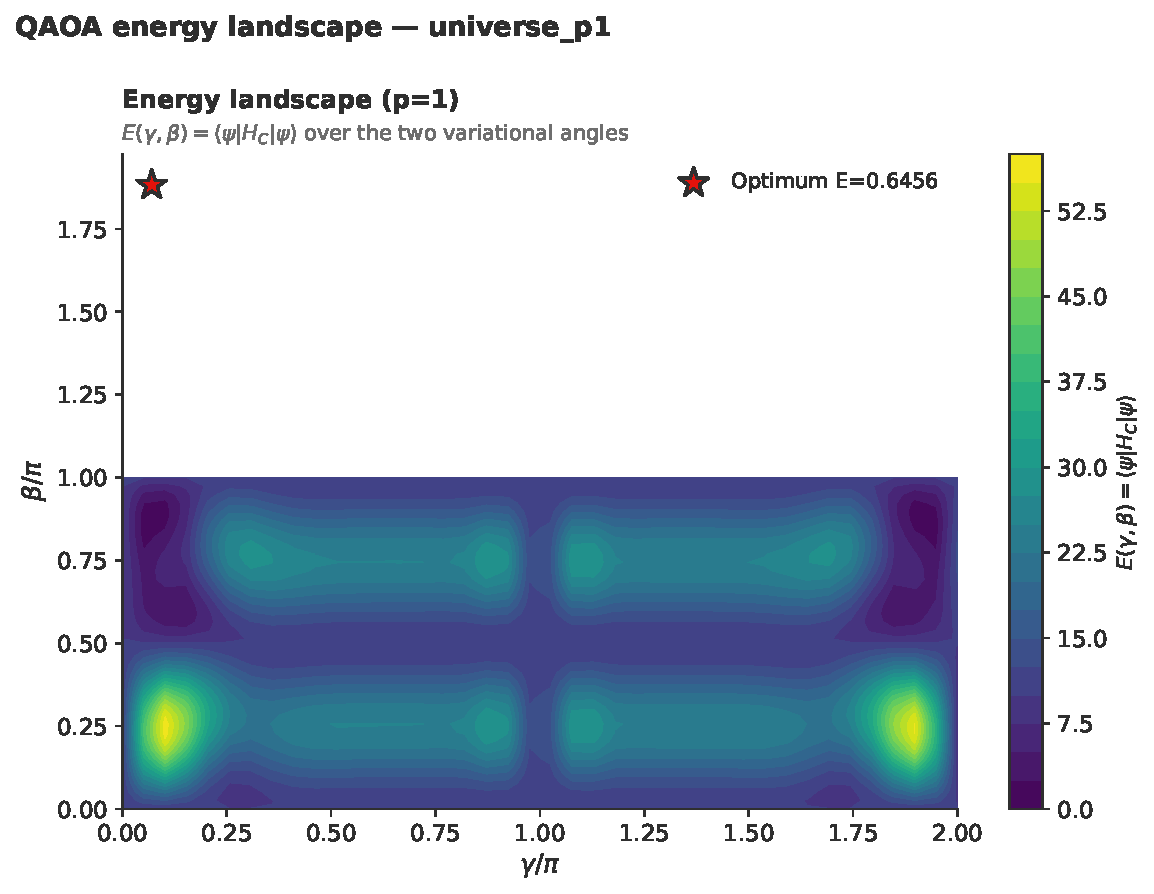
\includegraphics[width=0.8\textwidth]{plots/analysis/universe_p1_landscape.pdf}
    \caption{QAOA energy landscape $E(\gamma,\beta) = \langle\psi(\gamma,\beta)|H_C|\psi(\gamma,\beta)\rangle$ at $p=1$ on the canonical instance ($n=16$, $K=4$, $\lambda=2.0$, $A=0.5$), evaluated on a uniform grid over $(\gamma/\pi, \beta/\pi) \in [0,2]\times[0,2]$. The red star marks the best of ten COBYLA multi-starts, at $E = 0.6456$.}
    \label{fig:landscape}
\end{figure*}

The surface is visibly $\pi$-periodic in $\gamma$ and exhibits a small number of broad basins separated by saddles; the energy varies by roughly two orders of magnitude across the grid, from $E \sim 50$ in the bright hot-spots near $(\gamma/\pi, \beta/\pi) \approx (0, 0.25)$ to the small basins in the corners where the COBYLA optimum at $E = 0.65$ lives. The $\pi$-periodicity is a structural fingerprint of the cost Hamiltonian: the phase-separation unitary $e^{-i\gamma H_C}$ phases each basis state by $\exp(-i\gamma C(\boldsymbol{x}))$, and the QUBO coefficients of \cref{eq:Qcoeffs} are dominated by the integer-valued penalty terms $A(1-2K) = -3.5$ and $2A = 1.0$, so the half-integer effective quantum induces a $\pi$-period that the small continuous return/risk corrections from $(\boldsymbol\mu, \boldsymbol\Sigma)$ only mildly blur. Two practical consequences follow. First, the basins of attraction at $p=1$ are broad enough that ten random COBYLA starts hit the right neighbourhood reliably, in line with the shallow-QAOA landscape analysis of \textcite{zhou2018qaoa} and with the single-run figure above. Second, at $p \geq 2$ the surface lives in $\mathbb{R}^{2p}$ and the same multi-start budget covers it exponentially less densely; by $p=3$ the search volume has grown by a factor of roughly $(2\pi)^4 \approx 1.5 \times 10^3$ relative to $p=1$. This sets up the depth sweep in the next subsection, where the non-monotone behaviour in $r$ from $p \geq 3$ onwards should be read as the angle space outgrowing a fixed restart budget rather than as a failure of the ansatz itself.


\subsection{Circuit depth $p$}\label{subsec:sp-depth-results}

Does deeper circuit ansatz monotonically improve the approximation ratio, as the original QAOA analysis of \textcite{farhi2014qaoa} would suggest in the noiseless limit? \Cref{fig:depth-sweep} sweeps $p \in \{1,\dots,5\}$ on the canonical instance, with everything else held fixed.

\begin{figure*}[t]
    \centering
    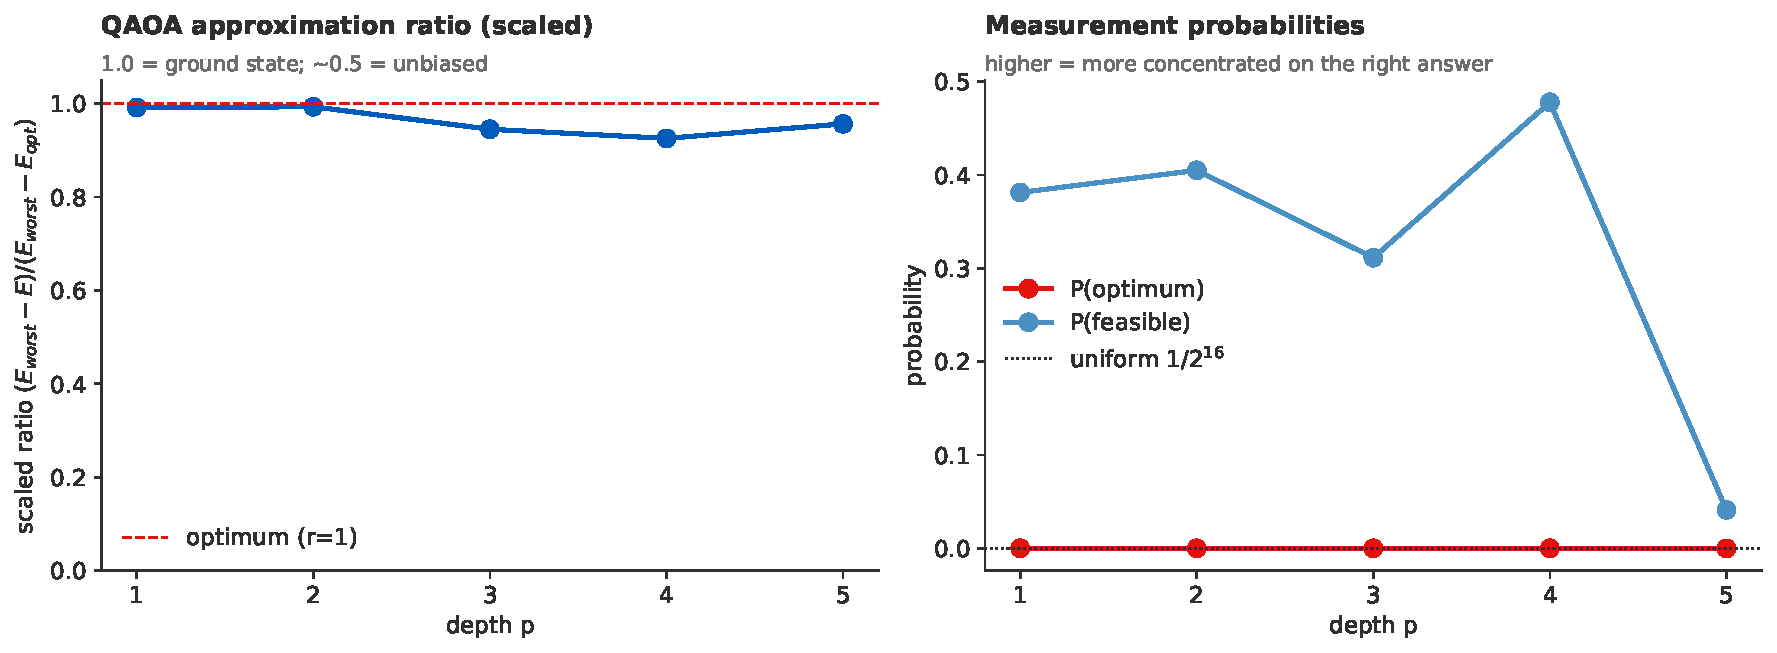
\includegraphics[width=0.8\textwidth]{plots/compare/depth_sweep.pdf}
    \caption{Depth sweep on the canonical instance ($n=16$, $K=4$, $\lambda=2.0$, $A=0.5$, ten COBYLA multi-starts per $p$, statevector backend). Left: scaled approximation ratio $r$ versus circuit depth $p$, with the brute-force reference at $r=1$ shown as a dashed line. Right: top-1 success probability $p_{\text{opt}}$ and feasibility probability $p_{\text{feas}}$ versus $p$, with the uniform-sampling baseline $1/2^{16}$ for context.}
    \label{fig:depth-sweep}
\end{figure*}

The observed sequence is non-monotonic. The ratio rises gently from $r = 0.991$ at $p=1$ to $0.993$ at $p=2$, then falls to $0.945, 0.925, 0.956$ at $p=3,4,5$. The unscaled gap tells a sharper version of the same story, moving from $461$ at $p=1$ to $374$ at $p=2$ before exploding to $2847$, $3854$, and $2257$ at $p=3,4,5$. The top-1 probability stays in a narrow band $p_{\text{opt}} \in [1.4\times 10^{-5}, 2.1\times 10^{-4}]$ and the feasibility mass fluctuates $p_{\text{feas}} \in [0.04, 0.48]$ without a clear trend.

The non-monotonicity is best read as an optimiser pathology rather than a property of the QAOA ansatz: the variational landscape lives in $2p$ angles and at $p\geq 3$ that is six or more dimensions, which ten random COBYLA seeds cannot tile reliably. \textcite{zhou2018qaoa} showed that warm-starts derived from optimal $p-1$ angles essentially restore the monotone depth--quality scaling that the original QAOA bound of \textcite{farhi2014qaoa} predicts in the noiseless limit, and the pattern observed here --- a clean gain from $p=1$ to $p=2$ followed by collapse once the angle search becomes high-dimensional --- is the textbook signature of that diagnosis. The $p=5$ collapse in feasibility mass to $p_{\text{feas}} = 0.04$ suggests the best restart at that depth latched onto an infeasible local minimum whose penalised energy beats the feasible neighbours found by the other nine seeds. We retain $p=3$ as the canonical setting since it is the shallowest depth at which all sweeps were run, but caution that the apparent ``optimal'' depth is restart-budget dependent. The depth-vs-noise trade-off explored by \textcite{shen2025noisy} is moot here because the simulator is exact; on hardware, deeper circuits would also have to fight increasing two-qubit error per layer.


\subsection{Budget-penalty calibration $A$}\label{subsec:Asensitivity-results}

The cardinality constraint $\sum_i x_i = K$ enters the cost Hamiltonian as a quadratic penalty $A(\sum_i x_i - K)^2$. Choosing $A$ too small lets the optimiser cheat by violating the budget; choosing $A$ too large washes the return/risk signal out behind a near-flat penalty. \Cref{fig:penalty-sweep} sweeps $A$ over almost two decades at fixed $p=3$.

\begin{figure*}[t]
    \centering
    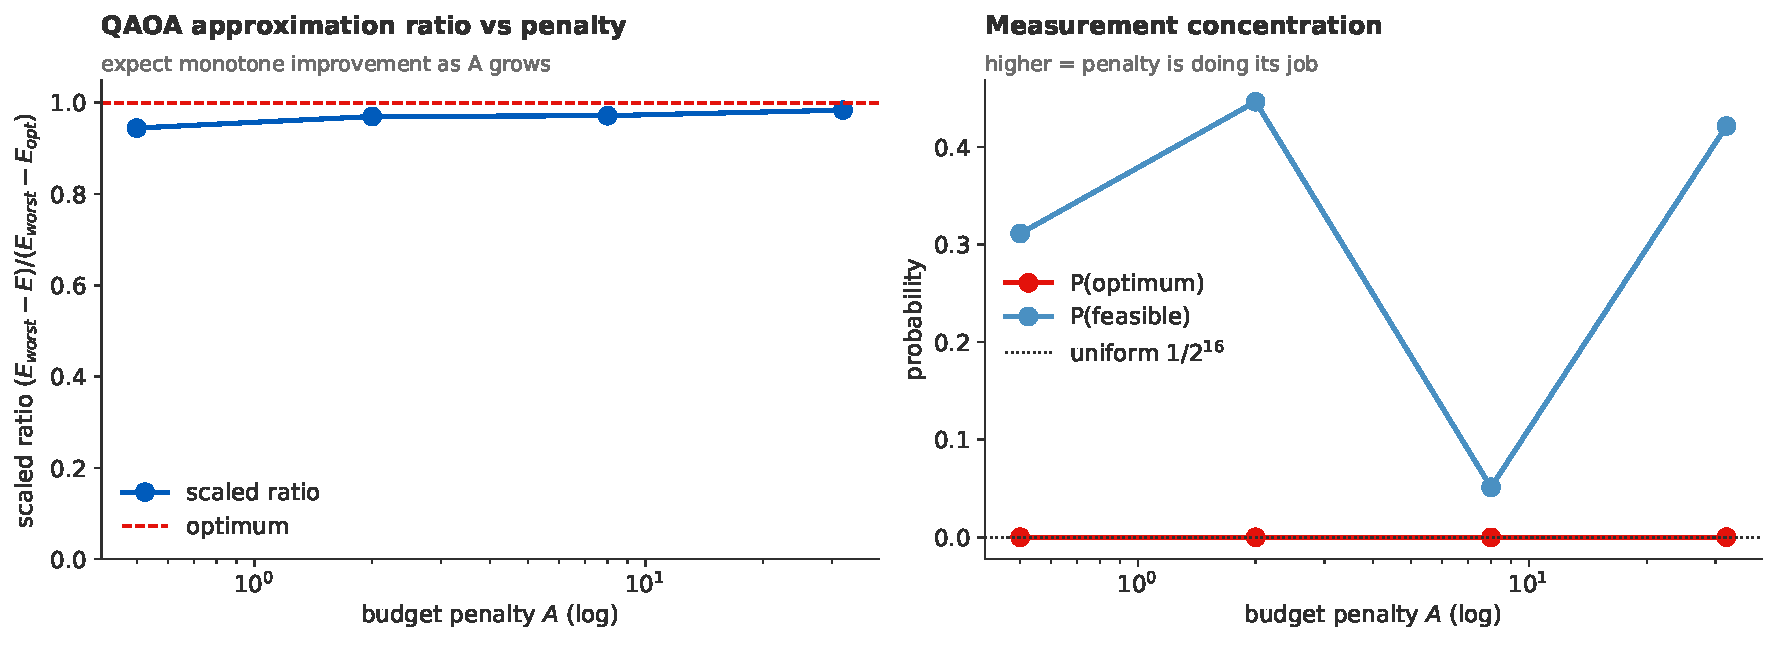
\includegraphics[width=0.8\textwidth]{plots/compare/penalty_sweep.pdf}
    \caption{Penalty sweep on the canonical instance ($n=16$, $K=4$, $p=3$, $\lambda=2.0$, ten COBYLA multi-starts per $A$, statevector backend). Left: scaled approximation ratio $r$ versus $A \in \{0.5, 2, 8, 32\}$ on a log axis. Right: top-1 success probability $p_{\text{opt}}$ and feasibility probability $p_{\text{feas}}$ versus $A$. The strong non-monotonicity in $p_{\text{feas}}$ reflects restart variance at a fixed ten-seed budget rather than a genuine signal in $A$.}
    \label{fig:penalty-sweep}
\end{figure*}

The scaled ratio creeps upward across the sweep: $r = 0.945, 0.970, 0.972, 0.984$ as $A$ moves through $0.5, 2, 8, 32$. This drift is mostly an artefact of the metric itself, because $(E_{\text{worst}}-E_{\text{opt}})$ scales linearly with $A$ via the worst basis state while the absolute gap grows by a much smaller factor; in the unscaled gap the sequence reads $2847, 6169, 23230, 52647$, so the variational state is moving further above the optimum in absolute terms, not closer to it. The feasibility mass $p_{\text{feas}}$ is non-monotone --- $0.31, 0.45, 0.05, 0.42$ --- with a striking collapse at $A=8$ that is almost certainly an unlucky COBYLA initialisation rather than a phase transition in the landscape.

The penalty sweep is therefore too coarse to identify an optimal $A$ and too noisy to read its derivative; the $p_{\text{feas}}$ trace would need an order of magnitude more restarts to become a reliable diagnostic, and even then would mostly track optimiser variance. The qualitative lesson points away from the penalty encoding altogether: the slack-variable construction of \textcite{thomassin2025slack} folds the budget into auxiliary qubits without a free coefficient, while a constraint-preserving XY-mixer in the spirit of \textcite{mancilla2026constrained} would dispense with $A$ entirely by restricting the search to the Hamming-weight-$K$ subspace. We did not run either experiment here, but the absence of a clean signal in $A$ is itself evidence that the choice was never going to be the lever it is sometimes presented as. For the remainder of this report we keep $A = 0.5$ on the grounds that it makes both metrics most interpretable and that the unscaled gap is smallest there.


\subsection{Risk-aversion $\lambda$}\label{subsec:risk-results}

The mean-variance objective $-\boldsymbol\mu^\top \boldsymbol{x} + \lambda\, \boldsymbol{x}^\top \boldsymbol\Sigma \boldsymbol{x}$ contains a single user-facing tuning knob, the risk-aversion $\lambda$. \Cref{fig:risk-sweep} traces the canonical solvers across seven log-spaced values $\lambda \in [10^{-1}, 10^{2}]$ at fixed $p=3$.

\begin{figure*}[t]
    \centering
    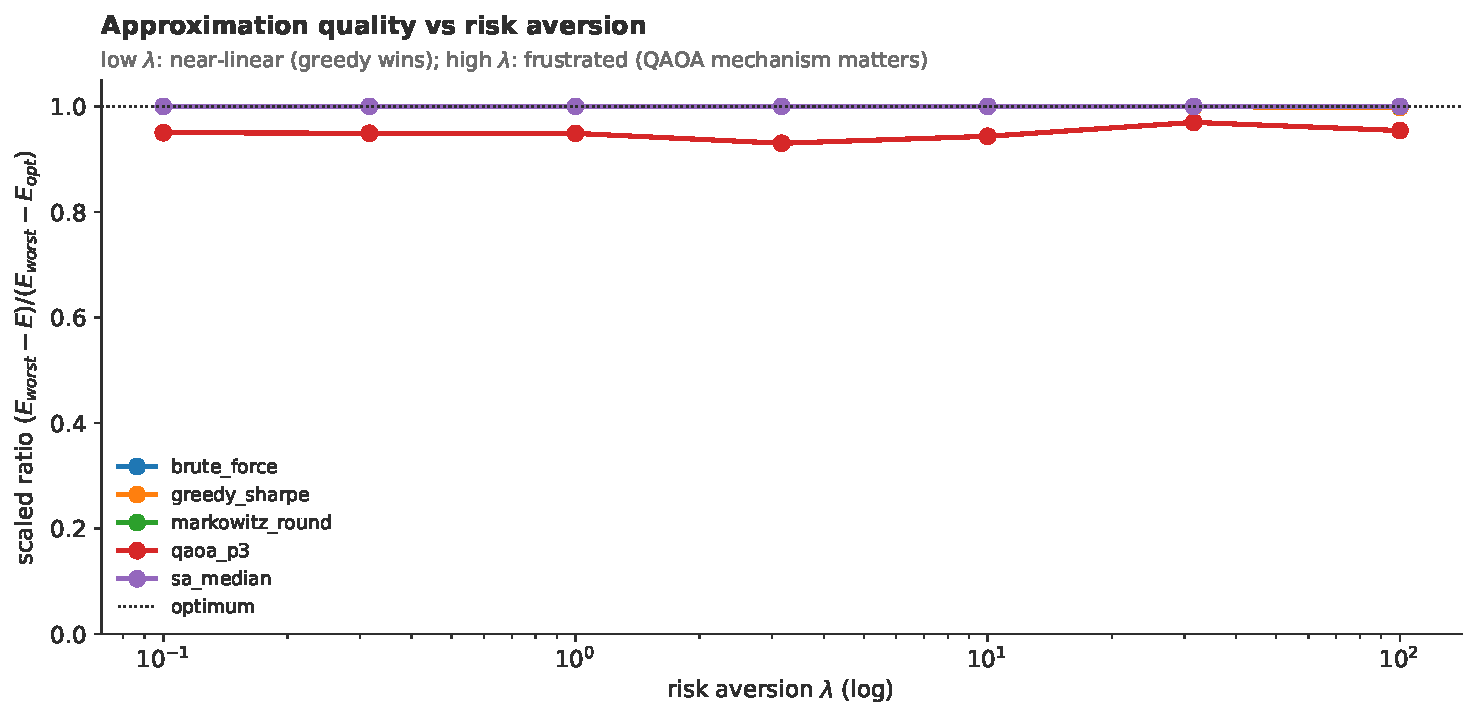
\includegraphics[width=0.8\textwidth]{plots/compare/risk.pdf}
    \caption{Risk-aversion sweep on the canonical instance ($n=16$, $K=4$, $p=3$, $A=0.5$, ten COBYLA multi-starts per $\lambda$). Scaled approximation ratio versus $\lambda$, log-spaced over three decades. Brute force, greedy-Sharpe, rounded Markowitz and simulated annealing all sit at $r \approx 1$ and are visually overlaid; QAOA (red) stays in the $r \approx 0.93$--$0.97$ band across the full sweep.}
    \label{fig:risk-sweep}
\end{figure*}

The four classical baselines --- brute force, greedy-Sharpe, rounded continuous Markowitz, and simulated annealing --- all sit at $r = 1$ to within numerical precision across the full $\lambda$ range. QAOA at $p=3$ trails them by a stable $0.03$--$0.07$ in the scaled ratio. The headline numbers across the sweep are $r_{\text{qaoa}} = 0.950, 0.949, 0.949, 0.930, 0.943, 0.970, 0.954$ for $\lambda = 0.1, 0.316, 1, 3.16, 10, 31.6, 100$ respectively; the unscaled gap is uniformly large but tracks the absolute scale of the objective, which itself drifts with $\lambda$. The top-1 mass is unaffected, oscillating between $3\times 10^{-5}$ and $2\times 10^{-4}$ throughout.

That QAOA is $\lambda$-insensitive at this resolution is informative: the algorithm's quality is bottlenecked by the depth/restart budget, not by the relative weight of return vs.\ variance in the objective. The dip at $\lambda = 3.16$ to $r = 0.930$ recovers at the next sweep value and is best read as another instance of the restart-variance pathology that dominated the $A$-sweep. In contrast, the rounded Markowitz baseline does begin to slip away from $r=1$ at the extreme tails of the sweep, indicating that the continuous relaxation provides a less informative starting point when the objective is dominated by variance ($\lambda \to \infty$) or by return ($\lambda \to 0$); even there, however, its ratio remains above $0.999$, far better than QAOA's $0.94$--$0.97$ band. This rules out a simple ``$\lambda$ was just unlucky'' explanation of the QAOA gap and re-focuses attention on the ansatz and its optimiser rather than on the objective.


\subsection{Problem size $n$ and classical baselines}\label{subsec:scaling-results}

How do the solvers compare as the problem size grows from $n=4$ to $n=16$, and is there any operating point where QAOA is competitive? \Cref{fig:scaling,fig:scaling-zoom} answer this question on five solvers and seven problem sizes.

\begin{figure*}[t]
    \centering
    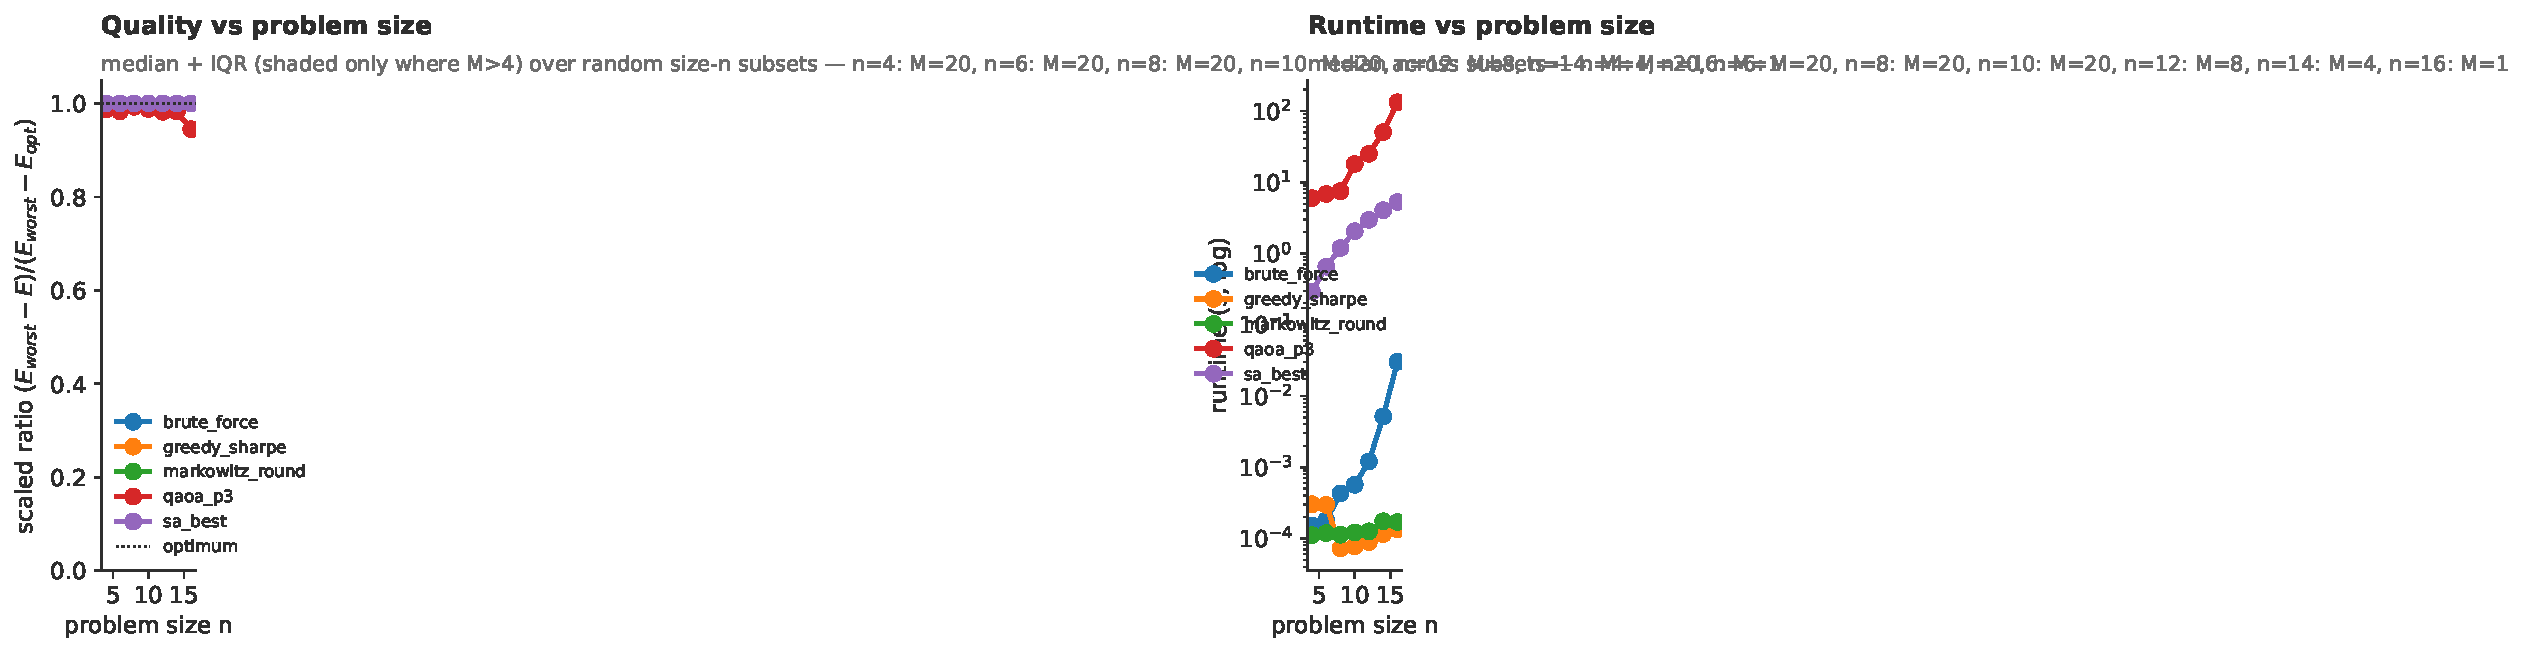
\includegraphics[width=0.8\textwidth]{plots/compare/scaling.pdf}
    \caption{Size scaling on random subsets of the canonical universe (target cardinality $K = 1, 2, 2, 2, 3, 4, 4$ for $n = 4, 6, 8, 10, 12, 14, 16$ respectively; $\lambda = 2.0$, $A = 0.5$, QAOA at $p=3$ with ten COBYLA multi-starts). Median over $M$ random subsets per problem size: $M=20$ for $n \in \{4,6,8,10\}$, $M=8$ for $n=12$, $M=4$ for $n=14$ and $M=1$ for $n=16$ --- the last point is a single instance and should be read as a sanity check rather than an estimate. Left: scaled approximation ratio per solver vs $n$. Right: median wall-clock runtime in seconds on a log axis; QAOA grows roughly as $2^n$ from circuit simulation cost while greedy-Sharpe, rounded Markowitz and brute force stay below tens of milliseconds.}
    \label{fig:scaling}
\end{figure*}

\begin{figure*}[t]
    \centering
    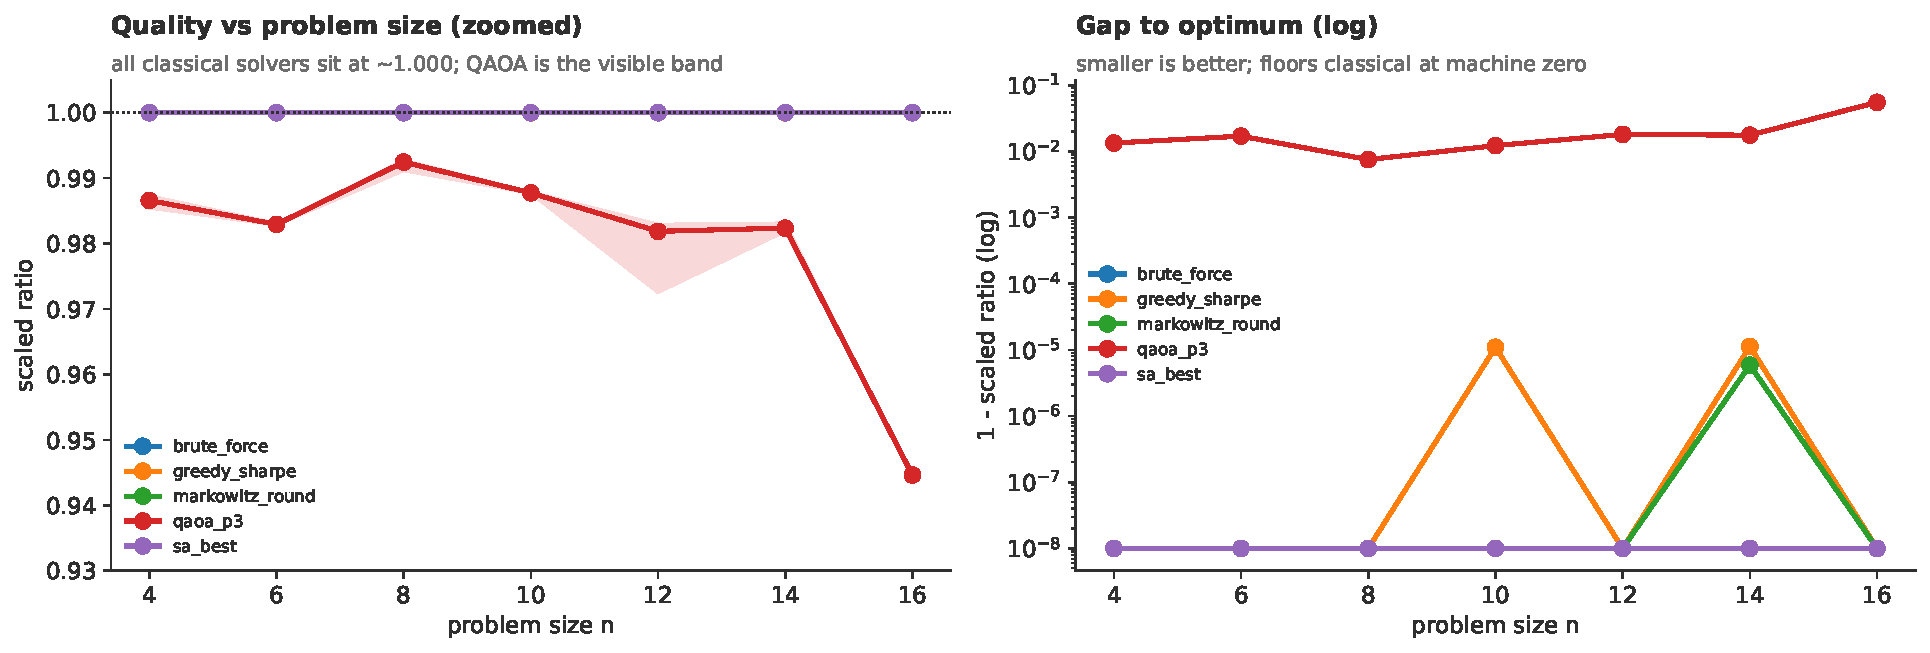
\includegraphics[width=0.8\textwidth]{plots/compare/scaling_zoom.pdf}
    \caption{Same sweep as \cref{fig:scaling}, zoomed to expose the QAOA-vs-classical gap. Left: scaled ratio restricted to $r \in [0.93, 1.00]$. Right: $1-r$ on a log axis; the classical solvers floor near floating-point zero, while QAOA stays in the $10^{-2}$--$10^{-1}$ band across all $n$.}
    \label{fig:scaling-zoom}
\end{figure*}

The classical baselines are essentially indistinguishable from brute force on these instances: median $r = 1$ for greedy-Sharpe, rounded Markowitz and simulated annealing at every $n$ tested, with $\mathrm{gap}$ at floating-point zero. QAOA at $p=3$ trails them: median $r$ takes the values $0.987, 0.983, 0.993, 0.988, 0.982, 0.982, 0.945$ for $n = 4, 6, 8, 10, 12, 14, 16$. The trend is mild in the scaled metric but stark in the top-1 mass, which collapses geometrically from $0.23$ at $n=4$ through $0.030$ at $n=8$ and $1.7\times 10^{-3}$ at $n=12$ to $1.6\times 10^{-4}$ at $n=16$. The per-step ratios fluctuate between $2\times$ and $6\times$, broadly tracking the growth of $\binom{n}{K}$ from $4$ at $n=4,\,K=1$ to $1820$ at $n=16,\,K=4$: the QAOA distribution at $p=3$ asymptotes towards uniformity over the feasible subspace rather than concentrating on the optimum, an outcome consistent with the cardinality-constrained QAOA findings of \textcite{knapsack2024qaoa}.

Runtimes complete the picture. Median brute-force wall-clock grows from $0.15$ ms at $n=4$ to $30$ ms at $n=16$; greedy-Sharpe and rounded Markowitz stay below $0.2$ ms across the entire range; simulated annealing rises from $0.29$ s at $n=4$ to $5.3$ s at $n=16$ at its default iteration budget. QAOA grows from $6$ s at $n=4$ to $132$ s at $n=16$, dominated by the $O(2^n)$ statevector cost. At the largest size, brute force is $\sim 4400\times$ faster than QAOA and reaches machine-precision optimality; there is no operating point on this benchmark where QAOA wins on either axis.

This is in line with the noiseless-vs-noisy comparisons of \textcite{shen2025noisy}: on classically tractable instances classical heuristics dominate. The methodological value of running QAOA here lies in the characterisation of its mechanism --- depth dependence, restart variance, $p_{\text{opt}}$ scaling --- not a competitive runtime. Looking forward, the Pauli-decomposition strategy of \textcite{soloviev2025pauli} suggests how to scale beyond $n=16$ without paying the full $O(2^n)$ simulator cost, but reaching the regime where the variational bound of \textcite{tilly2022vqe} becomes non-trivially tight will require constraint-preserving mixers, warm-starts, or both. Annealing comparisons \parencite{morapakula2025annealing} would also be informative on instances large enough to escape exact diagonalisation.


\subsection{Summary}\label{subsec:results-summary}

The five sweeps converge on a consistent picture. On the canonical $n=16$ instance at $p=3$ the QAOA pipeline reaches $r = 0.945$, but the absolute energy is $2847\times$ the optimum, the top-1 mass is only ten times the uniform baseline, and a brute-force enumeration solves the same instance to numerical precision in $30$ ms against QAOA's $132$ s. The depth and penalty sweeps show that the ansatz is more sensitive to optimiser luck than to its own hyper-parameters at the ten-restart budget used here; the risk sweep shows that $\lambda$ is not the bottleneck; the size sweep shows that the top-1 success probability decays as $1/\binom{n}{K}$, consistent with a near-uniform distribution over feasible bitstrings rather than a concentration on the optimum. The headline numbers are collected in \cref{tab:results-summary}.

\begin{table}[H]
    \centering
    \caption{Headline numbers on the canonical $n=16$ instance at $p=3$, $K=4$, $\lambda=2.0$, $A=0.5$, ten COBYLA multi-starts. Brute-force wall-clock is the same canonical instance, single-thread Python on the same machine; QAOA wall-clock is total time across all restarts including statevector simulation.}
    \label{tab:results-summary}
    \begin{tabular}{@{}lr@{}}
        \toprule
        Metric & Value \\
        \midrule
        Scaled ratio $r$                       & $0.945$ \\
        Relative gap $\mathrm{gap}$            & $2847$ \\
        Top-1 mass $p_{\text{opt}}$            & $1.6\times 10^{-4}$ \\
        Feasibility mass $p_{\text{feas}}$     & $0.31$ \\
        QAOA wall-clock                        & $132$ s \\
        Brute-force wall-clock                 & $0.03$ s \\
        \bottomrule
    \end{tabular}
\end{table}
